\newpage
\section{Реализация симулятора}

Главной частью работы является программное обеспечение для моделирования
массива. Основным краеугольным камнем можно считать быстродействие системы, 
так как одним из требований к конечному продукту была работа в реальном масштабе
времени. Основной интерфейс программы выполнен в минималистичном стиле, управление
камерой производится с помощью мыши, отображаемые слои выставляются с клавиатуры.

\vspace{1em}

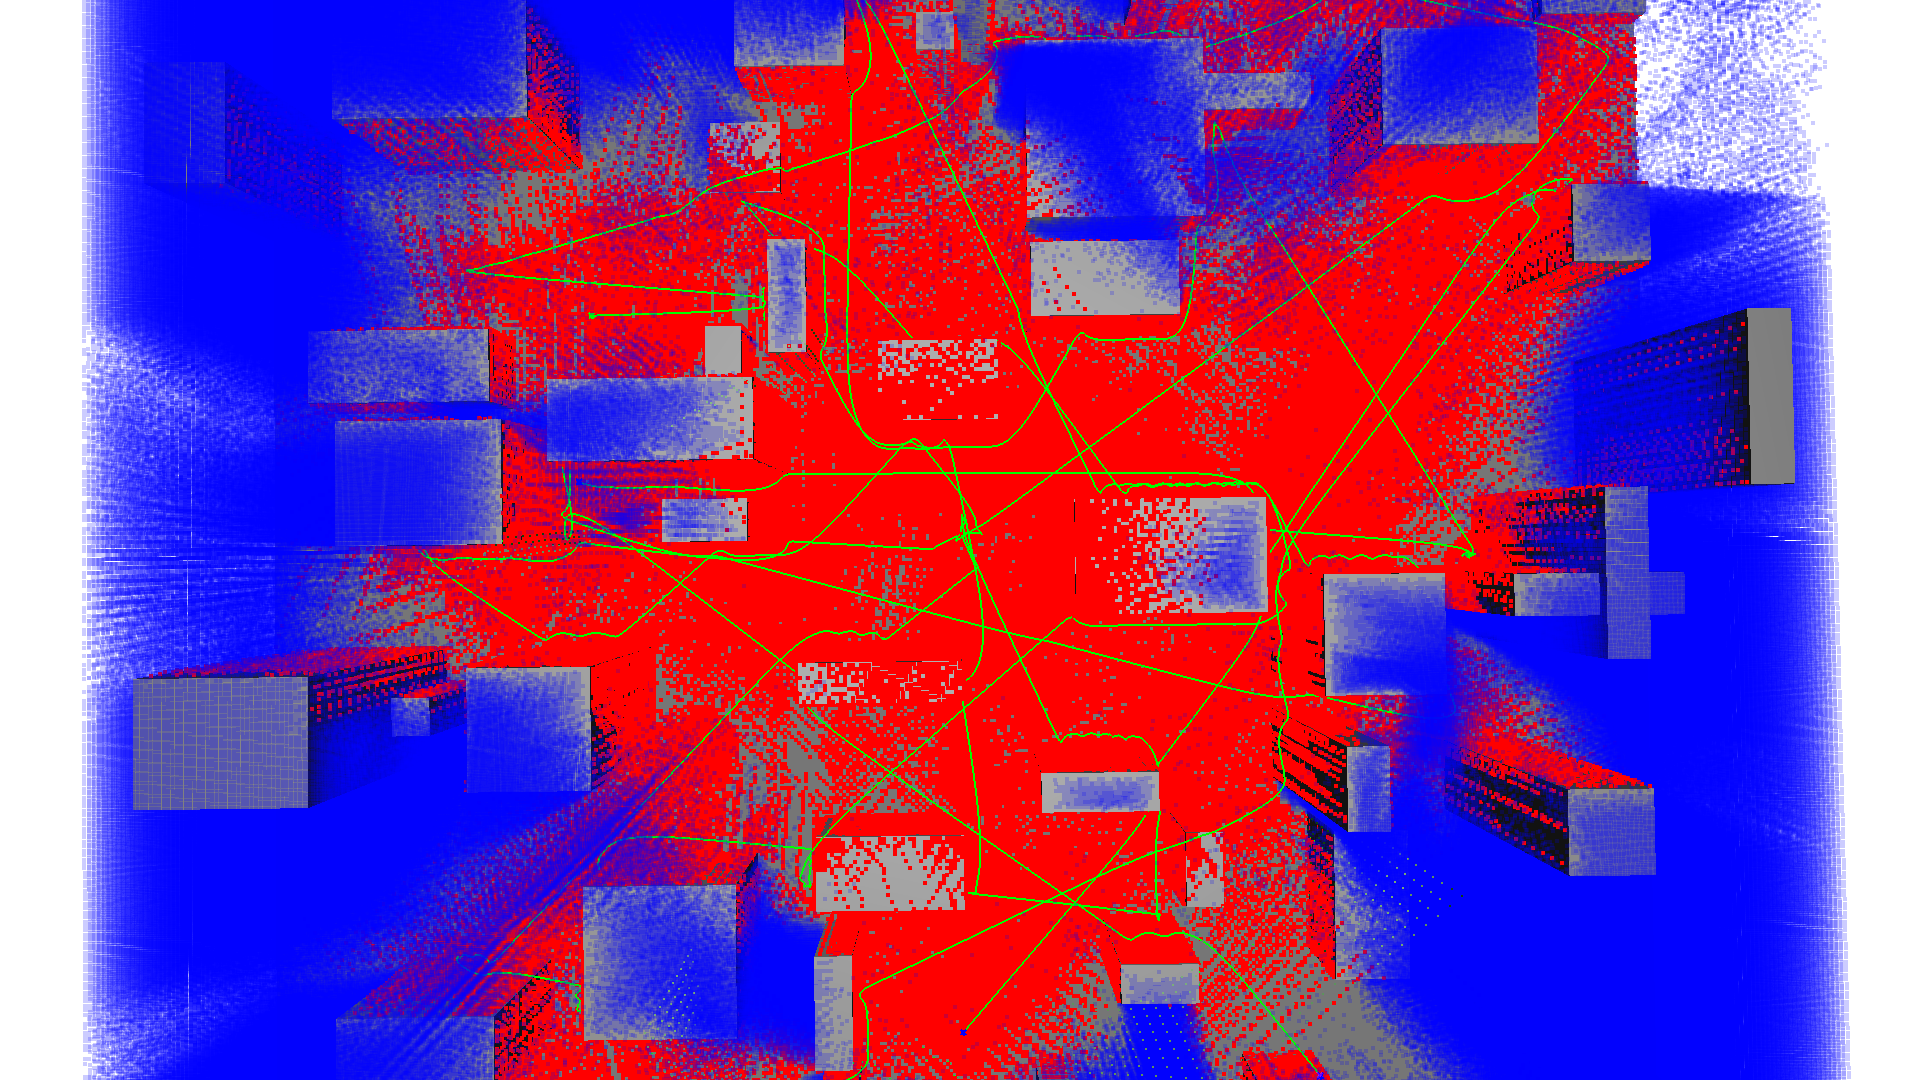
\includegraphics[width=\linewidth]{pa4.png}

ПО разрабатывалось на языке программирования D\footnote{компилируемый, С-подобный
язык программирования со статической типизацией}. Операционная система, используемая
при разработке Linux(Fedora).

Код проекта доступен по URL: \verb|https://github.com/deviator/dplm|.

\newpage
\subsection{Модель карты местности}

На данном этапе выполнения работы было решено хранить информацию о местности в
виде дискретной карты с ограничениями по высоте, глубине и ширине. Карта
представляет из себя массив прямоугольных секторов, хранящих фиксированный объём
информации:
\begin{mintemize}
    \item факт обследованности
    \item наличие объекта
\end{mintemize}

Реализация карты представляет собой 1-мерный массив, к которому можно обратиться с помощью трёх
индексов-координат.

Правила перевода индекса в координаты и обратно:

\nextverbatimspread{1}
\begin{verbatim}
    z = index / ( width * height )
    tmp = index % ( width * height )
    y = tmp / width
    x = tmp % width

    index = z * width * height + y * width + x
\end{verbatim}
\vspace{-0.5em}

где:

\verb|a / b| -- целочисленное деление \verb|a| на \verb|b|;

\verb|a % b| -- остаток от деления \verb|a| на \verb|b|;

\verb|index| -- индекс в одномерном массиве;

\verb|width| -- ширина поля;

\verb|height| -- высота поля;

\verb|x,y,z| -- координаты по ширине, высоте и глубине соответственно.

Также для карты имеется матрица трансформации координат из локальных (индексов)
в глобальные (метры).

При разрешении карты $400 \times 400 \times 50$ получаем $8 \cdot 10^6$ секторов.
Обработку таких объёмов данных было решено производить с помощью гетерогенных 
вычислений на GPU. Была использована технология \verb|OpenCL|. Это так же 
позволяет решить вопрос отображения данных через \verb|OpenGL|, так как
интероперабельность с графической системой использует zero-copy память -- 
физически это один участок памяти для буферов \verb|OpenCL| и \verb|OpenGL|.

\newpage
\subsection{Модель единицы массива}

За основу была взята концепция БПЛА с вертикальным взлётом (коптер или вертолёт),
то есть юнит имеет возможность зависать в точке и резко изменять направление движения.

На данном этапе работы математическая модель движения юнита очень проста:
$$
\left\{
    \begin{array}{l l}
    \dot{\vec{p}}  & = \vec V \\
    \dot{\vec{V}}  & = \vec a + \vec g
    \end{array}
\right.
$$

где:

$\vec p = (x,y,z)^T$ -- координаты юнита,

$\vec V = (V_x,V_y,V_z)^T$ -- скорость юнита,

$\vec a$ -- ускорение, вычисленное, как сумма всех сил делённая на массу,

$\vec g$ -- ускорение свободного падения,

$$ \vec a = \frac{1}{m} \cdot limit \left( \sum_{i=0}^N \vec f_N \right) $$

где:

$m$ -- масса юнита,

$limit \left( \vec f \right)$ -- вектор-функция, представляющая ограничение
по максимальной тяге двигателей юнита;

$\vec f_N$ -- управляющие силы.

К списку управляющих сил, в данной реализации алгоритма, относятся: 
\vspace{-0.5em}
\begin{mintemize}
    \item $\vec f_{\text{тр}} = -\vec V \cdot |V| \cdot C_x \cdot S \cdot \rho / 2$ -- сила трения о воздух,

    \item $\vec f_{\text{п}} = (0,0,-9.81 \cdot m)^T$ -- константная сила, компенсирующая силу тяжести,
        введена в архитектурных целях (в дальнейшем планируется изменить модель юнита
        для большей схожести с квадрокоптером)

    \item $\vec f_{\text{ц}}$ -- сила, реализующая движение к заданной точке
    \item $\vec f_{\text{к}}$ -- коррекция по ближайшим юнитам и точкам карты, ближе определённого расстояния
\end{mintemize}

Список сил возможно будет меняться в процессе реализации нового функционала, либо при переработке старого.

\newpage
Примерный код функции $limit \left( \vec f \right)$:

\nextverbatimspread{1}
\begin{verbatim}
    vec3 limit( vec3 f )
    {
        if( f.xy.len > max_horisontal_force )
            f.xy = f.xy.e * max_horisontal_force;
        if( f.z > max_up_force ) f.z = max_up_force;
        if( f.z < min_up_force ) f.z = min_up_force;
        return f;
    }
\end{verbatim}

где:

\verb|f.xy| -- вектор, составленный из компонент вектора \verb|f|,

\verb|f.xy.len| -- длина вектора,

\verb|f.xy.e| -- единичный вектор.

Такой алгоритм обрезки максимальной тяги позволяет в горизонтальной плоскости двигаться к цели прямолинейно,
а выход на требуемую высоту происходит максимально быстро.

\newpage
\subsection{Модель измерителей и заполнение карты}

Предполагается что каждый юнит имеет возможность
оценить дальность в любом направлении, в нескольких точках одновременно с определённым 
угловым разрешением (карта глубин).

Каждый юнит получает информацю о мире с помощью датчика глубины в виде картинки,
где каждому пикселю соответствует измерение дальности в определённых угловых координатах. В работе не эмулировлись
дистрозийные искажения, поэтому для приведения карты глубин в точки в системе координат юнита достаточно 
матрицы перспективной трансформации, которая имеется у каждого юнита. Она также может меняться в процессе работы
системы при необходимости (изменение угла обзора, зум). Строится эта матрица так:

$$
M_{persp} = \left( \begin{array}{c c c c}
        \frac{1}{ R \cdot \tan( \frac{1}{2} A ) } & 0 & 0 & 0 \\
        0 & \frac{1}{ \tan( \frac{1}{2} A ) } & 0 & 0 \\
        0 & 0 & \frac{ z_{n} + z_{f} }{ z_{n}-z_{f} } & \frac{ 2 \cdot z_{n} \cdot z_{f} }{ z_{n} - z_{f} } \\
        0 & 0 & -1 & 0
\end{array} \right)
$$

где:

$R = \frac{w}{h}$ -- соотношение сторон изображения

$A$ -- угол обзора по вертикали

$z_{n}$ -- дальность от центра камеры до ближней плоскости отсечения

$z_{f}$ -- дальность от центра камеры до дальней плоскости отсечения

При трансформации точки с помощью перспективной матрицы координаты результирующей точки
получаются в диапазоне $x \in [-1,1]$, $y \in [-1,1]$, $z \in [0,1]$. Все точки, что выходят
за эти пределы, не отображаются. Для работы с четырёхменой матрицей необходимо использовать
однородные координаты.

Переход от однородных координат к декартовым: 

\verb|vec3 C = U.xyz / U.w|

Переход от декартовых к однородным:

\verb|vec4 U = vec4( C.xyz, 1 )|

где:

\verb|U| -- четырёхмерный вектор однородных координат,

\verb|C| -- трёхмерный вектор в декартовых координатах.

\newpage

Процесс получение карты глубин реализован посредством \verb|OpenGL|. Для этого 
производится рендеринг мира в Frame Buffer, где для карты глубин выставлена текстура, 
которая потом копируется в буфер \verb|OpenCL|. Копирование из текстуры в буфер реализованно
из-за ограничений \verb|OpenCL 1.1|. Прямое использование изображений с глубиной добавленно
только в стандарте \verb|OpenCL 2.0|, вышедшем в 2013г. Драйвер видеокарты на рабочей машине
не поддерживал последний стандарт.

Точки имеют дополнительную информацию -- было ли что-либо найдено.
Это вычисляется с так: \verb|bool finded = depth[iy*w+ix] < 1.0f - 1e-6;|.
То есть, если значение глубины крайне близко к максимальному, можно считать, что
луч из камеры не наткнулся ни на один объект.

После получения точек в связанной системе координат они приводятся
сначала к мировой, затем к системе координат карты.
Так же приводится положение юнита (камеры) к системе координат карты.

Заполняется карта по следующему алгоритму:
\begin{mintemize}
    \item строится отрезок из точки камеры (А) к точке, полученной с датчика (Б)
    \item все сектора, которые находятся между А и Б помечаются как исследованные
    \item сектор, в котором находится точка с датчика помечается как заполненый,
        если в ней было что-то найдено.
\end{mintemize}

\newpage
\subsection{Логика перемещения юнитов}

Для системы в целом ставится задача полностью исследовать объём, отражаемый в карте.
Из этого следует, что каждый юнит направляется к ближайшему неизведанному участку.

Указание маршрута следования юниту даётся через так называемые целевые точки.
Их расстановка высчитывается совместно для всего массива. Первая итерация расчёта
случайная. На следующих итерациях расстановка происходит по следующему алгоритму:
\begin{mintemize}
\item для фиксированных объёмов карты (прямоугольные области) вычисляется суммарное
    количество неизведанных точек
\item выбирается область с максимальным количеством неизвестных точек
\item проверяется назначен ли этот объём другому юниту:
    \begin{mintemize}
        \item если нет, целевая точка назначается в центр области
        \item если назначен, выбрать вторую (и далее), по количеству неизвестных точек область
    \end{mintemize}
\item при достижении целевой точки юнит расчитывает следующую целевую точку
\end{mintemize}

Размер прямоугольных областей карты выбирается, исходя из максимальной дальности работы
датчика глубины юнита, и составляет удвоенное её значение.

\newpage
\subsection{Алгоритм перемещения юнитов}

Важно, чтобы юниты не сталкивались друг с другом и не врезались в стены.
На данный момент реализация коррекции движения производится через аддитивное управляющее
воздействие $f_{\text{к}}$. 

Алгоритм вычисления $f_{\text{к}}$:
\begin{mintemize}
\item координаты заполненных точки карты совмещают в массив с координатами юнитов
\item выбираются только те точки, что ближе к юниту чем $D_{min}$
\item для каждой точки вычисляетются 2 составляющие $f_{\text{к}}$: нормальная и тангенсальная
\item складываются результаты
\end{mintemize}

\tikzstyle{every picture}+=[
    axis/.style={black},
    vector/.style={->,thick,black},
    help/.style={gray,thin,dashed},
    rot/.style={tdplot_rotated_coords}
]

\begin{center}

    \def\dot{circle[radius=0.5mm]}
    \def\P{1.9}
    \def\Pm{1.6}
    \def\Pmm{0.5}
    \def\Vrot{20}
    \def\fnlen{5}
    \def\ftlen{2}
    \def\dst{8}

    \tdplotsetmaincoords{0}{0}
    \begin{tikzpicture}[tdplot_main_coords]
        \tdplotsetrotatedcoords{85}{60}{-50}
        \fill[rot,red] (\dst,  0,  0) \dot;
        \fill[rot,red] (\dst, .5,  0) \dot;
        \fill[rot,red] (\dst,-.5,  0) \dot;
        \fill[rot,red] (\dst, .5, .5) \dot;
        \fill[rot,red] (\dst,-.5, .5) \dot;
        \fill[rot,red] (\dst,  0, .5) \dot;
        \fill[rot,red] (\dst,  0,-.5) \dot;
        \fill[rot,red] (\dst, .5,-.5) \dot;
        \fill[rot,red] (\dst,-.5,-.5) \dot;

        \fill[rot,black] (0,0,0) \dot node[below] {$O$};

        \draw[rot,vector] (0,0,0) -- (\dst,0,0);
        \node[rot,above] at (6,0,0) {$\vec D$};
        \draw[rot,vector] (0,0,0) -- (1,0,0);
        \node[rot,below] at (1,0,0) {$\vec e_D$};

        \draw[rot,vector] (0,0,0) -- (\Vrot:5) node[above] {$\vec V$};
        \draw[rot,vector] (0,0,0) -- (\Vrot:1) node[above] {$\vec e_V$};
        \draw[rot,vector,help] (0,0,0) -- (0,0,3);
        \node[rot,left] at (0,0,3) {$\vec U$};
        \draw[rot,vector,red] (0,0,0) -- (-\fnlen,0,0);
        \draw[rot,vector,red] (0,0,0) -- (-1,0,0);
        \node[rot,below left] at (-\fnlen,0,0) {$\vec f_N$};
        \node[rot,below] at (-1,0,0) {$\vec N$};
        \draw[rot,vector,green] (0,0,0) -- (0,\ftlen,0);
        \draw[rot,vector,green] (0,0,0) -- (0,1,0);
        \node[rot,above left] at (0,\ftlen,0) {$\vec f_T$};
        \node[rot,above] at (0,1,0) {$\vec T$};
        \draw[rot,vector,blue] (0,0,0) -- (-\fnlen,\ftlen,0);
        \node[rot,above left] at (-\fnlen,\ftlen,0) {$\vec f_{\text{к}}$};

        \draw[rot,help] (0,\ftlen,0) -- ++(-\fnlen,0,0) -- ++(0,-\ftlen,0);

        \draw[rot,help] (0,0,\P) -- ++(0:\P) -- ++(0,0,-\P);
        \draw[rot,help] (0,0,\P) -- ++(\Vrot:\P) -- ++(0,0,-\P);
        \draw[rot,help] (0,\Pm,0) -- ++(\Pm,0,0) -- ++(0,-\Pm,0);
        \draw[rot,help] (-\Pmm,0,0) -- ++(0,\Pmm,0) -- ++(\Pmm,0,0);
    \end{tikzpicture}

\end{center}

На рисунке:

$O$ -- положение юнита,

$\vec D$ -- расстояние до точки,

$\vec e_D = \frac{\vec D}{|\vec D|}$ -- еденичный вектор расстояния,

$\vec V$ -- скорость юнита,

$\vec e_V = \frac{\vec V}{|\vec V|}$ -- еденичный вектор скорости юнита,

$\vec U = \vec e_D \times \vec e_V$ -- промежуточный вектор,

$\vec T = normalize(\vec U \times \vec e_D)$ -- направление тангенсальной коррекции

$\vec N = -\vec e_D$ -- направление нормальной коррекции.

\newpage
Коррекция $\vec f_{\text{к}}$ вычисляется по формуле:

$$\vec f_{\text{к}} = ( ( \vec N \cdot ( D_{min} - |D| )^2 \cdot K_1 + \vec T ) \cdot max( K_2, < \vec e_D, \vec e_V > ) ) \cdot K_3 $$

где:

$K_{[1,2,3]}$ -- эмпирически подобранные коэффициенты, 

$< \vec e_D, \vec e_V >$ -- скалярное произведение.

Коэффициент $(D_{min} - |D|)^2$ увеличивается квадратично,
при пересечии юнитом минимально допустимой дистанции. Это позволяет
резко остановить юнит при прямом сближении с опасной точкой.

Коэффициент $max(0, < \vec e_D, \vec e_V > )$ обращается в ноль в случае,
если юнит двигается от опасной точки, и становится равным единице в случае,
если юинт имеет направление ровно на опасную точку. Это позволяет уменьшить
отталкивание от стен при паралельном движении вдоль них. Коэффициент $K_2$ оставляет
минимальное отталкивание от стены и ускорение вдоль стены, даже в случае, если
юнит движется от стены. Направление по коррекции по скорости позволяет лучше
обходить препятсвтия, нежели в случае направления по вектору дальности до цели.

Коэффициент $K_3$ позволяет подавлять управляющее воздействие по целевой \lb точке.
